\documentclass[border=3pt]{standalone}
\usepackage{tikz}
\usetikzlibrary{arrows.meta,calc,positioning}
\tikzset{pin/.style={-{Stealth[length=5pt]}},
  blk/.style={draw, thick, font=\sffamily\small, align=center}}
\begin{document}
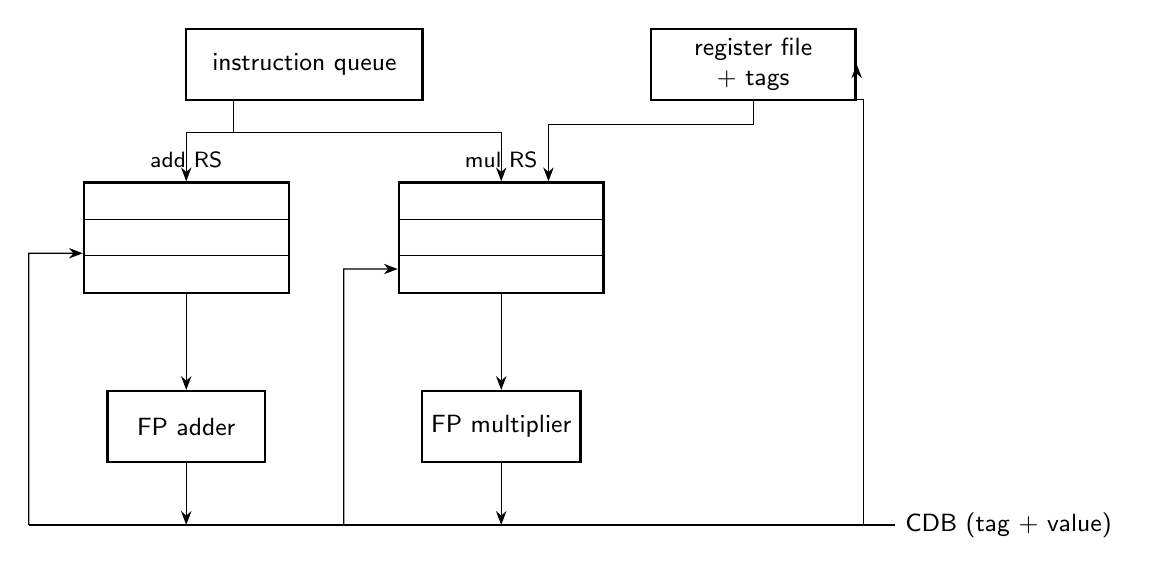
\begin{tikzpicture}[font=\sffamily\small]
  \node[blk, minimum width=30mm, minimum height=9mm] (iq) at (2.9,3.1) {instruction queue};
  \node[blk, minimum width=26mm, minimum height=9mm] (rf) at (8.6,3.1) {register file\\+ tags};
  % reservation stations
  \node[blk, minimum width=26mm, minimum height=14mm] (rs1) at (1.4,0.9) {};
  \node[font=\sffamily\footnotesize, above=0.5mm of rs1.north] {add RS};
  \node[blk, minimum width=26mm, minimum height=14mm] (rs2) at (5.4,0.9) {};
  \node[font=\sffamily\footnotesize, above=0.5mm of rs2.north] {mul RS};
  \foreach \n in {rs1,rs2}{\foreach \y in {-2.33,2.33}{\draw ($(\n.west)+(0,\y mm)$) -- ($(\n.east)+(0,\y mm)$);}}
  % dispatch
  \draw[pin] (iq.south) ++(-0.9,0) |- ++(0,-4mm) -| (rs1.north);
  \draw[pin] (iq.south) ++(-0.9,0) |- ++(0,-4mm) -| (rs2.north);
  \draw[pin] (rf.south) -- ++(0,-3mm) -| ($(rs2.north)+(6mm,0)$);
  % functional units
  \node[blk, minimum width=20mm, minimum height=9mm] (fu1) at (1.4,-1.5) {FP adder};
  \node[blk, minimum width=20mm, minimum height=9mm] (fu2) at (5.4,-1.5) {FP multiplier};
  \draw[pin] (rs1.south) -- (fu1.north);
  \draw[pin] (rs2.south) -- (fu2.north);
  % CDB
  \draw[thick] (-0.6,-2.75) -- (10.4,-2.75) node[right, font=\sffamily\small]{CDB (tag + value)};
  \draw[pin] (fu1.south) -- (1.4,-2.75);
  \draw[pin] (fu2.south) -- (5.4,-2.75);
  % CDB feeds back
  \draw[pin] (10.0,-2.75) -- ++(0,5.4) -| (rf.east) ;
  \draw[pin] (-0.6,-2.75) -- ++(0,3.45) -- ($(rs1.west)+(0,-2mm)$);
  \draw[pin] (3.4,-2.75) -- ++(0,3.25) -- ($(rs2.west)+(0,-4mm)$);
\end{tikzpicture}
\end{document}
